%% Elsevier cas-dc double-column manuscript
%% Sections 1-3 (Introduction / Theoretical background / Proposed method)
%% drafted for the CMGAN-T60 (Fourier-KAN) paper.

\documentclass[a4paper,fleqn]{cas-dc}

\usepackage[numbers]{natbib}
\usepackage{amsmath}
\usepackage{amssymb}
\usepackage{graphicx}
\usepackage{booktabs}
\usepackage{multirow}
\usepackage{url}

%% Author definitions
\def\tsc#1{\csdef{#1}{\textsc{\lowercase{#1}}\xspace}}

\begin{document}
\let\WriteBookmarks\relax
\def\floatpagepagefraction{1}
\def\textpagefraction{.001}

\shorttitle{Conformer-based blind $T_{60}$ estimation with Fourier-KAN regression head}
\shortauthors{X. Xie et~al.}

\title[mode=title]{Conformer-based blind reverberation time estimation with a Fourier Kolmogorov--Arnold regression head}

%% ------------- Authors (placeholder) -------------
\author[1]{Xinni Xie}[%
  type=editor,
  orcid=0000-0000-0000-0000]
\cormark[1]
\ead{xiexinni@example.edu}

\affiliation[1]{organization={TODO Department, TODO University},
                city={TODO},
                country={TODO}}

\cortext[cor1]{Corresponding author}

\begin{abstract}
% TODO: rewrite abstract once Sections 4--6 are in place.
Reverberation time $T_{60}$ is one of the most informative room-acoustic
parameters, yet blind estimation from a single-channel noisy reverberant
recording remains difficult because the late reverberation tail is easily
masked by additive noise. We propose a single-task $T_{60}$ estimation
network that combines a dual-path time--frequency Conformer encoder with
a lightweight Fourier Kolmogorov--Arnold network (Fourier-KAN) regression
head. The complex short-time Fourier
spectrum of the noisy reverberant utterance is processed by a dense
convolutional encoder followed by two time--frequency Conformer blocks
(TSCBs), and the resulting bottleneck features are aggregated by a
multi-statistic pooling layer before being mapped to $T_{60}$ by a
two-layer Fourier-KAN head. Compared with a multi-layer perceptron head of
similar capacity, the Fourier basis expresses each univariate activation as
a learnable trigonometric series, which is well matched to the smooth but
non-linear dependence between pooled acoustic statistics and the target
$T_{60}$. Experiments on four noisy reverberant test sets covering both
simulated and measured room impulse responses, with seen and unseen noise
types, show that the proposed model attains an average root-mean-squared
error of $111.2$\,ms, a mean absolute error of $72.4$\,ms and a Pearson
correlation of $0.948$.
\end{abstract}

\begin{keywords}
Blind reverberation time estimation \sep Conformer \sep Kolmogorov--Arnold
network \sep Fourier basis \sep Noise robustness \sep Speech enhancement
\end{keywords}

\maketitle

% =====================================================================
\section{Introduction}
% =====================================================================

When a sound is emitted in an enclosure, the receiver captures not only
the direct path but also a dense set of reflections from the surrounding
boundaries~\citep{kuttruff2013room}. These reflections decay over time and
together form the room reverberation. The time required for the sound
energy to decay by 60\,dB after the source has been switched off is
defined as the reverberation time $T_{60}$~\citep{iso3382_2_2008}. As a
single scalar that summarises the energy-decay behaviour of a room,
$T_{60}$ is one of the most widely used parameters to characterise the
acoustic property of an enclosure and has a direct impact on speech
quality, intelligibility, and the performance of downstream audio
applications such as dereverberation, speech recognition, sound source
localisation, and virtual or augmented reality
rendering~\citep{benzeghiba2007asrreview, anthes2016vr}. The standardised
ways of measuring $T_{60}$ are the interrupted-noise method and the
integrated impulse response method~\citep{schroeder1965rt}, both of which
require omnidirectional sources, calibrated microphones and trained
operators. Such site-measurement campaigns are not portable and are
prohibitively expensive whenever large-scale or in-situ measurements are
needed, which motivates the so-called \emph{blind} setting, in which
$T_{60}$ is inferred directly from a recorded speech signal without any
dedicated excitation or knowledge of the room
geometry~\citep{eaton2016ace}.

Over the past two decades, a large body of work on blind $T_{60}$
estimation has accumulated. The traditional family relies on statistical
signal processing: model-based estimators describe the late part of the
room impulse response (RIR) as a damped Gaussian
process~\citep{polack1988these} and recover $T_{60}$ from the decay rate
of the energy envelope, while feature-mapping based estimators derive
$T_{60}$ from a hand-designed acoustic descriptor such as the negative-side
variance of the decay rate, the pitch strength of harmonic
components or the spectral decay
distribution~\citep{ratnam2003blind, wen2008negativeside, eaton2013sdd,
falk2010temporal, lollmann2010iwaenc}. These methods have been thoroughly
benchmarked by the ACE challenge~\citep{eaton2016ace}, which also revealed
two recurring difficulties: (i) most estimators are positively biased by
additive noise because the noise-like reverberation tail is buried in the
noise, and (ii) the analytic decay model is fragile in non-stationary or
low-SNR scenarios. Even noise-robust extensions such as the
spectral-decay-distribution estimator with reduced computational
cost~\citep{eaton2013sdd} or the subband-decomposition based
estimator~\citep{prego2015subband} still require a relatively accurate
prior estimate of the noise level, which is itself a hard problem when
the noise is non-stationary.

Deep learning (DL) has subsequently emerged as a data-driven alternative.
\citet{gamper2018cnn} fed log-mel features to a six-layer convolutional
neural network and won the ACE single-channel track; \citet{xiong2018ercnn}
posed the joint $T_{60}$ and direct-to-reverberant ratio estimation as a
classification problem on time--frequency features; \citet{deng2020crnn}
introduced a convolutional recurrent network for online estimation on
variable-length utterances; \citet{srivastava2021blindroom} extended the
formulation to multi-channel inputs; \citet{goetz2023online} tackled
parameter estimation under dynamic acoustic conditions with three
convolutional recurrent variants; \citet{zheng2022noiseaware} and
\citet{zhang2024damtl} explored multi-task formulations that pair $T_{60}$
regression with an auxiliary denoising objective; and more recently
\citet{saini2023mobileaudiotransformer} have demonstrated that a
MobileViT-style transformer can run on a smartphone in real time, while
\citet{duangpummet2022stochastic} have moved from full-band $T_{60}$
towards a joint estimation of $T_{60}$, early-decay time, clarity and
speech transmission index. Although these data-driven models clearly
outperform the statistical signal processing baselines in clean or
high-SNR conditions, two general challenges persist across this body of
work. First, the late reverberation tail is intrinsically energy-weak
and is easily masked by real-world noise, so estimation accuracy still
degrades noticeably in low-SNR or unseen-noise scenarios. Second, almost
all existing estimators place a stack of fully connected layers on top
of the temporal/spectral backbone as the regressor, which applies a
single fixed non-linearity per neuron and offers limited expressive
power for the smooth but non-trivial mapping from pooled bottleneck
statistics to a scalar $T_{60}$.

To address these challenges, we adopt time--frequency Conformer
blocks~\citep{gulati2020conformer, cao2022cmgan} as the encoder
backbone: self-attention is applied along the time and frequency axes
in a dual-path fashion, which captures the long temporal context and
frequency-dependent spectral coupling that characterise late
reverberation. As the regression head, we adopt a Fourier-basis
Kolmogorov--Arnold network (Fourier-KAN)~\citep{liu2024kan,
xu2025fourierkan, yang2025kanforspeech}, whose learnable univariate
edge functions replace the fixed scalar non-linearities of an MLP and
supply a strong inductive bias toward the smooth low-dimensional
regression from pooled bottleneck statistics to $T_{60}$. To the best
of our knowledge, neither building block has previously been deployed
in a blind $T_{60}$ estimator.

\noindent\textbf{Contributions.} Building on these observations, this
paper proposes a single-task $T_{60}$ estimation framework that combines
a dual-path time--frequency Conformer encoder with a Fourier-KAN
regression head. Our specific contributions are as follows.

\begin{enumerate}[(1)]
  \item We design a dual-path time--frequency Conformer encoder for
        single-task blind $T_{60}$ estimation. A three-channel complex
        STFT representation (magnitude, real and imaginary parts) is
        first projected by a dense convolutional front-end, and the
        resulting bottleneck features are then refined by two stacked
        two-stage Conformer blocks that alternate self-attention along
        the time and frequency axes. To the best of our knowledge,
        such a dual-path time--frequency attention encoder has not
        previously been explored for blind $T_{60}$ regression.
  \item We design a lightweight Fourier-KAN regression head. The encoder
        bottleneck features are first averaged along the frequency axis
        and aggregated along the time axis by a multi-statistic pooling
        layer (average, maximum and standard deviation). The pooled
        embedding is projected and normalised, then fed to a two-layer
        Fourier-KAN block in which the first layer uses a larger number of
        frequency components than the inner layers. A final linear
        projection and a sigmoid map the result to a normalised $T_{60}$.
        The head adds about $86$\,k parameters and the entire network
        contains approximately $0.86$\,M parameters; despite this
        compact footprint, the proposed head consistently outperforms
        an MLP head of comparable size.
  \item We carry out a systematic evaluation on four noisy reverberant
        test sets covering all combinations of simulated/measured RIRs and
        seen/unseen noise types, with the input SNR sampled from
        $\{0,5,10,15,20\}$\,dB. The proposed model attains an average
        RMSE of $111.2$\,ms, an MAE of $72.4$\,ms and a Pearson
        correlation of $0.948$, and ablation studies confirm that the
        Conformer backbone and the Fourier-KAN head each contribute a
        statistically significant share of the improvement.
\end{enumerate}

The remainder of this paper is organised as follows. Section~\ref{sec:bg}
formalises the acoustic signal model and reviews the classical and
data-driven approaches to blind $T_{60}$ estimation. Section~\ref{sec:method}
describes the proposed network in detail, including the Conformer
backbone, the multi-statistic pooling layer, the Fourier-KAN head and
the training objective. Section~\ref{sec:exp} presents the datasets, baselines and
implementation details. Section~\ref{sec:results} reports the
quantitative results and ablation studies, and Section~\ref{sec:conclusion}
concludes the paper.

% =====================================================================
\section{Theoretical background}\label{sec:bg}
% =====================================================================

\subsection{Acoustic signal model}\label{sec:bg:signal}

Let $s(t)$ be the anechoic speech emitted by a stationary source,
$h(t)$ the room impulse response (RIR) from the source position to the
microphone, and $n(t)$ the uncorrelated additive noise captured at the
microphone. In the time domain, the recorded noisy reverberant signal
$y(t)$ is modelled as the linear convolution of the source and the
RIR, contaminated by the noise~\citep{kuttruff2013room}:
\begin{equation}\label{eq:time_model}
  y(t) = s(t)\ast h(t) + n(t),
\end{equation}
where $\ast$ denotes the convolution operator and the noise-free
reverberant component is denoted by $x(t) = s(t)\ast h(t)$. In a realistic
setting the noise itself is typically reverberant, but with a different
RIR from $h(t)$~\citep{zheng2022noiseaware}.

Applying a short-time Fourier transform (STFT) with frame index $l$ and
frequency-bin index $k$ to Eq.~\eqref{eq:time_model} yields
\begin{equation}\label{eq:stft_model}
  Y(k,l) = X(k,l) + N(k,l) \approx S(k,l)\,H(k,l) + N(k,l),
\end{equation}
where $Y$, $X$, $S$, $H$ and $N$ denote, respectively, the STFTs of the
noisy reverberant signal, the noise-free reverberant signal, the clean
speech, the RIR and the additive noise. The blind $T_{60}$ estimation
task investigated in this paper is to learn a mapping
$\mathcal{F}:Y \mapsto \hat{T}_{60}$ that takes only the complex STFT of
the recorded signal as input, without access to $X$, $S$, $H$ or $N$.

\subsection{Reverberation time}\label{sec:bg:rt}

The reverberation time $T_{60}$ refers to the time required for the
sound pressure level to decrease by 60\,dB after the source has been
switched off~\citep{iso3382_2_2008}. A classical model-based way to
relate $T_{60}$ to the structure of the RIR is the Polack
model~\citep{polack1988these}, which describes the late RIR as a damped
zero-mean Gaussian process,
\begin{equation}\label{eq:polack}
  h(t) = b(t)\, e^{-\delta t},\qquad t\geq 0,
\end{equation}
where $b(t)$ is a stationary, independent and identically distributed
sequence with variance $\sigma_b^{2}$, and $\delta>0$ is the damping
constant of the room. From the second-order statistics of
Eq.~\eqref{eq:polack} the squared energy envelope decays as
\begin{equation}\label{eq:envelope}
  \mathbb{E}\{|h(t)|^{2}\} = \sigma_b^{2}\,e^{-2\delta t},
\end{equation}
and the reverberation time can be obtained in closed form as
\begin{equation}\label{eq:t60_from_delta}
  T_{60} = \frac{3\ln 10}{\delta}.
\end{equation}
This equation is the theoretical basis of many model-based estimators:
the decay rate $\delta$ is fitted to the logarithm of the (estimated)
energy envelope by a linear regression. When the reverberant speech is
contaminated by noise, the energy envelope is no longer a pure
exponential and the estimate of $\delta$ becomes severely biased,
typically yielding an over-estimation of
$T_{60}$~\citep{gaubitch2012comparison}.

A complementary point of view is offered by Sabine's empirical
formula~\citep{sabine1964papers}, which links $T_{60}$ to the room
volume $V$ and the average absorption $\bar{\alpha}$ of its surfaces of
total area $S$:
\begin{equation}\label{eq:sabine}
  T_{60} = \frac{0.161\,V}{\bar{\alpha}\,S},
\end{equation}
with the refinements of \citet{eyring1930reverberation} for high-absorption
rooms. Although Sabine's formula is not directly used for blind
estimation, it confirms that $T_{60}$ is a property of the room rather
than of the source, which justifies the use of $T_{60}$ as a single
scalar target for the regression network described in
Section~\ref{sec:method}.

\subsection{From statistical estimators to deep regression}\label{sec:bg:dl}

Prior blind $T_{60}$ estimators can be grouped into three broad
families:
\begin{enumerate}[(i)]
  \item \emph{Model-based estimators} fit a parametric decay model such
        as Eq.~\eqref{eq:envelope} to the energy envelope and derive
        $T_{60}$ from the estimated decay rate
        $\delta$~\citep{ratnam2003blind, lebart2001spectral,
        prego2012subband, hamza2016gamma}. They rely on the diffuse-field
        assumption and tend to break down in low-SNR scenarios.
  \item \emph{Feature-mapping estimators} extract a hand-crafted feature
        from the reverberant speech and learn a (typically polynomial)
        mapping to $T_{60}$. Examples include the negative-side variance
        of the decay rate distribution~\citep{wen2008negativeside}, the
        pitch strength of harmonic components~\citep{wu2006pitchstrength},
        spectro-temporal modulation features~\citep{falk2010temporal} and
        Mel-band spectral decay distributions~\citep{eaton2013sdd}.
  \item \emph{Deep regression estimators} replace both the feature
        extractor and the mapping by a neural network trained on a large
        corpus of simulated noisy reverberant
        speech~\citep{gamper2018cnn, xiong2018ercnn, deng2020crnn,
        srivastava2021blindroom, goetz2023online, saini2023mobileaudiotransformer,
        zheng2022noiseaware, zhang2024damtl}. The dominant architectural
        pattern is an encoder--regressor structure in which a
        convolutional or recurrent encoder extracts a fixed-size
        embedding from the spectrum and a fully connected regressor maps
        it to a scalar $T_{60}$.
\end{enumerate}

% =====================================================================
\section{Proposed method}\label{sec:method}
% =====================================================================

This section describes the proposed single-task $T_{60}$ estimation
network. As illustrated in Fig.~\ref{fig:overall} (placeholder), the
network is composed of three sub-blocks: (i) a complex-spectrum
\emph{feature encoder} that turns the noisy reverberant waveform into a
high-dimensional time--frequency representation; (ii) a dual-path
\emph{Conformer trunk} that captures long-range spectro-temporal
dependencies; and (iii) a Fourier-KAN \emph{regression head} that
aggregates the trunk output into a single normalised $T_{60}$ estimate.
The proposed network performs \emph{single-task} regression and does
not attempt to reconstruct any intermediate signal; the motivation for
this design choice is discussed in Section~\ref{sec:method:loss}.

\begin{figure*}[t]
  \centering
  % TODO: replace with the actual block diagram exported from the codebase.
  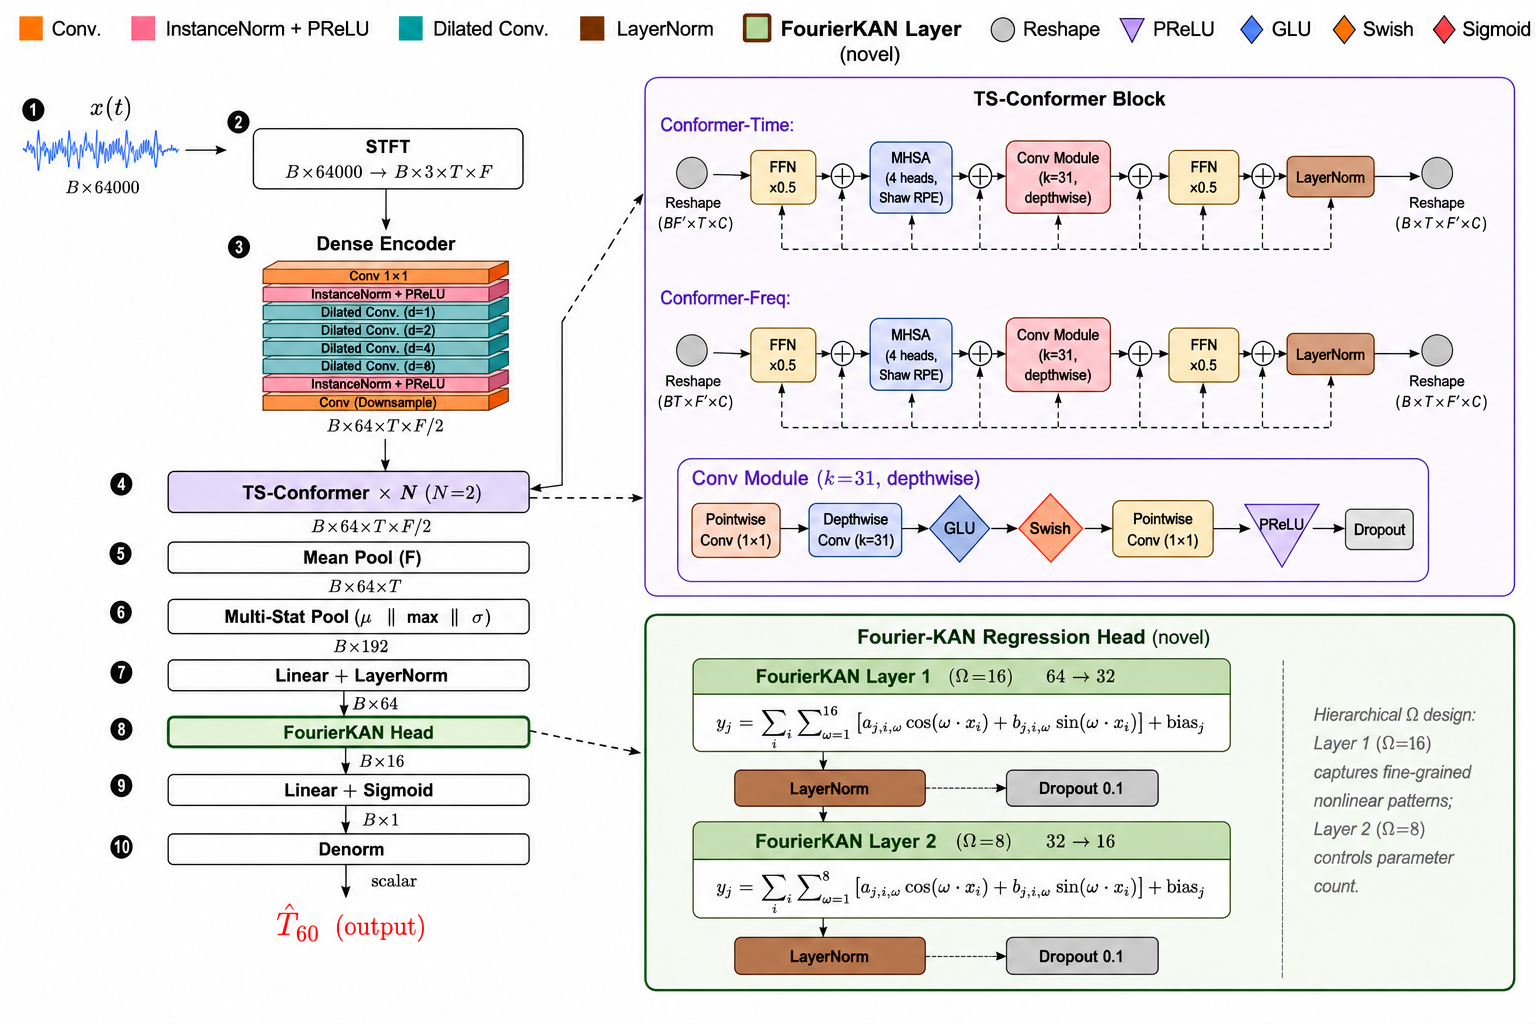
\includegraphics[width=0.95\textwidth]{figs/overall_architecture.pdf}
  \caption{Overview of the proposed Conformer-based $T_{60}$ estimation
  network with a Fourier-KAN regression head. Complex STFT features of
  the noisy reverberant utterance are processed by a dense convolutional
  encoder and two time--frequency Conformer blocks (TSCBs). The
  bottleneck feature map is averaged over the frequency axis, aggregated
  by a multi-statistic pooling layer over the time axis and mapped to
  $\hat{T}_{60}$ by a two-layer Fourier-KAN head.}
  \label{fig:overall}
\end{figure*}

\subsection{Input representation and pre-processing}\label{sec:method:input}

All recordings are resampled to $16$\,kHz, converted to mono and
truncated or padded to a fixed length of $4$\,s, yielding $L=64\,000$
samples per utterance. To make the input statistics independent of the
absolute recording level, each waveform $y[n]$ is scaled by an
energy-normalising factor
\begin{equation}\label{eq:energy_norm}
  c = \sqrt{\frac{L}{\sum_{n=0}^{L-1} y^{2}[n]+\varepsilon}},\qquad
  \tilde{y}[n] = c\,y[n],
\end{equation}
with $\varepsilon=10^{-8}$ added for numerical stability. The same
normalisation is applied at training and at inference time so that the
network never sees the raw signal level. A complex STFT is then
computed with a Hamming analysis window of $N=400$ samples and a hop
size of $H=100$ samples, yielding a complex spectrum
$\mathbf{Y}\in\mathbb{C}^{T\times F}$ of $T=641$ frames and $F=201$
frequency bins. The real and imaginary parts of $\mathbf{Y}$ are stacked
into a two-channel tensor and the magnitude $|\mathbf{Y}|=
\sqrt{\mathrm{Re}(\mathbf{Y})^{2}+\mathrm{Im}(\mathbf{Y})^{2}}$ is
concatenated as a third channel, producing the input tensor
\begin{equation}\label{eq:input_tensor}
  \mathbf{X}_{\mathrm{in}} = \bigl[\,|\mathbf{Y}|,\;
   \mathrm{Re}(\mathbf{Y}),\;\mathrm{Im}(\mathbf{Y})\,\bigr]
   \in\mathbb{R}^{3\times T\times F}.
\end{equation}
We deliberately avoid the power-law magnitude compression
$|\mathbf{Y}|^{p}$ commonly used in speech enhancement: $T_{60}$ is a
regression target that depends on the decay shape of the envelope rather
than on its instantaneous loudness, and the first convolutional layer
can learn a data-driven normalisation if needed.

\subsection{Dense convolutional encoder}\label{sec:method:encoder}

The encoder uses a dense convolutional design with three stages. A pointwise convolution first projects the
three-channel input to $C=64$ channels and is followed by instance
normalisation and a parametric ReLU. A \emph{dilated dense block} of
depth $D=4$ then applies four cascaded $2\times 3$ convolutions whose
inputs are formed by concatenating the outputs of all preceding
convolutions; the dilation rate of the $d$-th convolution along the time
axis is $2^{d-1}$, which exponentially enlarges the temporal receptive
field while keeping the parameter count under control. Each
convolution is followed by an instance normalisation and a PReLU
activation. Finally, a strided $1\times 3$ convolution downsamples the
frequency axis by a factor of two and produces the encoder bottleneck
\begin{equation}\label{eq:encoder}
  \mathbf{F}^{(0)} = \mathrm{Encoder}(\mathbf{X}_{\mathrm{in}})
        \in \mathbb{R}^{C\times T\times F'},
\end{equation}
with $C=64$, $T=641$ and $F'=101$.

\subsection{Two-stage Conformer trunk}\label{sec:method:tscb}

The Conformer block~\citep{gulati2020conformer} combines the global
modelling ability of self-attention with the local feature extraction
of convolutions, and has become a standard sequence-modelling choice
for speech enhancement and source separation. For a sequence
$\mathbf{Z}\in\mathbb{R}^{L\times d}$ of length $L$ and feature
dimension $d$, the block consists of four sub-modules wrapped in
residual connections:
\begin{equation}\label{eq:conformer}
  \begin{aligned}
    \mathbf{Z}_1 &= \mathbf{Z} + \tfrac{1}{2}\,\mathrm{FFN}_1(\mathbf{Z}),\\
    \mathbf{Z}_2 &= \mathbf{Z}_1 + \mathrm{MHSA}(\mathbf{Z}_1),\\
    \mathbf{Z}_3 &= \mathbf{Z}_2 + \mathrm{Conv}(\mathbf{Z}_2),\\
    \mathbf{Z}_4 &= \mathrm{LayerNorm}\bigl(\mathbf{Z}_3 +
                    \tfrac{1}{2}\,\mathrm{FFN}_2(\mathbf{Z}_3)\bigr),
  \end{aligned}
\end{equation}
where $\mathrm{FFN}_1$ and $\mathrm{FFN}_2$ are two pre-normalised
position-wise feed-forward modules with Swish activations,
$\mathrm{MHSA}$ is a multi-head self-attention module with Shaw-style
relative positional encoding~\citep{shaw2018relativepos}, and
$\mathrm{Conv}$ is a depth-wise separable 1-D convolution module with a
gated linear unit and a batch normalisation. The half-scaling of the two
feed-forward branches yields the so-called ``Macaron'' structure that
has been shown to stabilise optimisation~\citep{gulati2020conformer}.

When applied to a time--frequency representation of speech, the
Conformer block is typically deployed in a dual-path fashion: two
Conformer blocks are stacked, one operating along the time axis and one
along the frequency axis, jointly forming a two-stage Conformer block
(TSCB)~\citep{cao2022cmgan}. The encoder bottleneck $\mathbf{F}^{(0)}$
is then refined by $N=2$ stacked TSCBs. Concretely, for an input
feature map $\mathbf{F}\in\mathbb{R}^{B\times C\times T\times F'}$:
\begin{equation}\label{eq:tscb_time}
  \mathbf{F}^{t} = \mathbf{F}
      + \mathrm{ConformerBlock}_{t}\bigl(\mathrm{Reshape}_{t}(\mathbf{F})\bigr),
\end{equation}
where $\mathrm{Reshape}_{t}$ flattens the frequency axis into the batch
dimension and treats the time axis as the sequence axis; the Conformer
block then operates on tensors of shape $(B\,F')\times T\times C$.
Analogously,
\begin{equation}\label{eq:tscb_freq}
  \mathbf{F}^{tf} = \mathbf{F}^{t}
      + \mathrm{ConformerBlock}_{f}\bigl(\mathrm{Reshape}_{f}(\mathbf{F}^{t})\bigr),
\end{equation}
with $\mathrm{Reshape}_{f}$ producing tensors of shape $(B\,T)\times
F'\times C$. Each Conformer block has $h=4$ attention heads of dimension
$d_h=C/4=16$, a feed-forward expansion factor of $4$, a depth-wise
separable 1-D convolution with kernel size $31$, and a dropout rate of
$0.2$ on both the attention and the feed-forward sub-modules. After
the second TSCB, the bottleneck feature map is denoted
$\mathbf{F}^{(N)}\in\mathbb{R}^{C\times T\times F'}$. With $C=64$,
$T=641$ and $F'=101$, the per-block self-attention has quadratic
complexity in $T$ or $F'$ but only linear complexity in the product
$T\,F'$ thanks to the dual-path factorisation; this is what makes a
$4$-second window tractable on a single GPU.

\subsection{Frequency averaging and multi-statistic pooling}\label{sec:method:pool}

The Conformer trunk produces a four-dimensional feature map that has to
be condensed into a fixed-size embedding before regression. We adopt a
two-step pooling strategy. The frequency axis is first averaged, which
reflects the assumption that $T_{60}$ summarises a broadband property of
the room rather than a specific spectral pattern:
\begin{equation}\label{eq:freq_avg}
  \mathbf{Z}_{c,t} = \frac{1}{F'}\sum_{f=1}^{F'}\mathbf{F}^{(N)}_{c,t,f},
\end{equation}
yielding $\mathbf{Z}\in\mathbb{R}^{C\times T}$. The time axis is then
aggregated by a multi-statistic pooling layer that computes the average,
the maximum and the standard deviation along the time
dimension~\citep{snyder2018xvector}:
\begin{equation}\label{eq:multipool}
  \mathbf{e} = \bigl[\,\mu(\mathbf{Z}),\;
   \max(\mathbf{Z}),\;\sigma(\mathbf{Z})\,\bigr] \in \mathbb{R}^{3C}.
\end{equation}
The three statistics carry complementary information about the energy
envelope of the utterance: $\mu(\mathbf{Z})$ summarises the long-term
average level, $\max(\mathbf{Z})$ captures the peak excitation typically
associated with vowel onsets, and $\sigma(\mathbf{Z})$ captures the
temporal modulation of the envelope, which is known to be strongly
correlated with the decay rate of the late reverberation
tail~\citep{falk2010temporal}. With $C=64$, the resulting embedding has
$3C=192$ entries.

\subsection{Fourier-KAN regression head}\label{sec:method:head}

The Kolmogorov--Arnold representation theorem states that any
continuous multivariate function $f:[0,1]^{n}\to\mathbb{R}$ can be
written as the finite composition of univariate continuous functions
and addition. \citet{liu2024kan} build on this observation and propose
Kolmogorov--Arnold networks (KANs), in which the fixed scalar
non-linearities of a multi-layer perceptron (MLP) are replaced by
learnable univariate functions placed on every \emph{edge} of the
network. A single KAN layer with input dimension $I$ and output
dimension $O$ implements the mapping
\begin{equation}\label{eq:kan_layer}
  y_j = \sum_{i=1}^{I} \phi_{j,i}(x_i) + b_j,
  \qquad j=1,\ldots,O,
\end{equation}
where each $\phi_{j,i}:\mathbb{R}\to\mathbb{R}$ is a learnable univariate
function and $b_j$ is a per-output bias. The original KAN paper
parameterises $\phi_{j,i}$ by cubic B-splines, which is expressive but
requires bookkeeping such as adaptive grid updates and is comparatively
slow on small batch sizes typical of regression heads.

A Fourier-KAN replaces the spline basis by a truncated trigonometric
series~\citep{xu2025fourierkan, yang2025kanforspeech}. For a
\emph{frequency budget} $\Omega\in\mathbb{N}$, every edge function is
written as
\begin{equation}\label{eq:fourier_phi}
  \phi_{j,i}(x_i) = \sum_{\omega=1}^{\Omega}
    \bigl[a_{j,i,\omega}\,\cos(\omega\,x_i)
        + b_{j,i,\omega}\,\sin(\omega\,x_i)\bigr],
\end{equation}
so that the output of a Fourier-KAN layer becomes
\begin{equation}\label{eq:fourier_layer}
  y_j = \sum_{i=1}^{I}\sum_{\omega=1}^{\Omega}
        \bigl[a_{j,i,\omega}\cos(\omega x_i)
            + b_{j,i,\omega}\sin(\omega x_i)\bigr] + b_j.
\end{equation}
The number of trainable parameters per layer is $2\,O\,I\,\Omega + O$,
which is a modest multiple of an equivalent linear layer of size
$O\times I$ but still small in absolute terms when $I$ and $O$ are kept
small. Two properties make this basis attractive for the proposed
regression head: (i) gradients with respect to the weights are
closed-form trigonometric functions of the input and require no grid
maintenance; (ii) the basis has a strong inductive bias towards smooth
and approximately periodic dependencies, which matches the empirical
shape of the mapping from pooled bottleneck statistics to $T_{60}$.

The pooled embedding $\mathbf{e}\in\mathbb{R}^{192}$ is mapped to the
final estimate $\hat{T}_{60}$ by the Fourier-KAN head, depicted
in Fig.~\ref{fig:head} (placeholder). The head is composed of a linear
projection, a stack of two Fourier-KAN layers and a final linear output.
Each step is described below.

\paragraph{Projection.} A linear projection followed by a layer
normalisation reduces the pooled embedding to a $d_{0}=64$-dimensional
vector,
\begin{equation}\label{eq:proj}
  \mathbf{u}^{(0)} = \mathrm{LayerNorm}\bigl(\mathbf{W}_{p}\,\mathbf{e}+
                                              \mathbf{b}_{p}\bigr),
  \qquad \mathbf{u}^{(0)}\in\mathbb{R}^{d_{0}}.
\end{equation}
We intentionally omit any subsequent tanh activation: the layer
normalisation already controls the input range of the first Fourier
layer, while a tanh would saturate the periodic basis and waste capacity.

\paragraph{Fourier-KAN block.} The projected embedding is processed by
$L=2$ Fourier-KAN layers with hidden dimensions $(d_{1},d_{2})=(32,16)$.
The first layer uses a comparatively large frequency budget
$\Omega_{0}=16$, which allows it to learn fine-grained non-linear
features directly from the embedding, while the inner layer uses a
smaller budget $\Omega_{1}=8$ for parameter efficiency. Formally, for
$\ell=1,2$,
\begin{equation}\label{eq:fourier_block}
  u^{(\ell)}_j = \sum_{i=1}^{d_{\ell-1}}\sum_{\omega=1}^{\Omega_{\ell-1}}
    \bigl[a^{(\ell)}_{j,i,\omega}\cos(\omega u^{(\ell-1)}_i)
        + b^{(\ell)}_{j,i,\omega}\sin(\omega u^{(\ell-1)}_i)\bigr]
    + c^{(\ell)}_j,
\end{equation}
and the layer output is post-processed by a layer normalisation and a
dropout with probability $0.1$:
\begin{equation}\label{eq:fourier_post}
  \mathbf{u}^{(\ell)} \leftarrow \mathrm{Dropout}\bigl(
    \mathrm{LayerNorm}(\mathbf{u}^{(\ell)})\bigr).
\end{equation}
The Fourier weights $a^{(\ell)}_{j,i,\omega}$ and $b^{(\ell)}_{j,i,\omega}$
are initialised from a zero-mean Gaussian with standard deviation
$\sqrt{1/(d_{\ell-1}\,\Omega_{\ell-1})}$, so that the variance of the
layer output is approximately unity at initialisation regardless of the
input dimension and the frequency budget.

\paragraph{Output.} A linear layer maps $\mathbf{u}^{(2)}\in
\mathbb{R}^{16}$ to a scalar, and a sigmoid activation produces the
normalised estimate
\begin{equation}\label{eq:t60_hat}
  \hat{T}_{60}^{\mathrm{norm}} = \sigma\bigl(\mathbf{w}_{o}^{\top}\mathbf{u}^{(2)}
                                            + b_{o}\bigr) \in (0,1).
\end{equation}

\paragraph{Parameter budget.} With $(d_{0},d_{1},d_{2})=(64,32,16)$ and
$(\Omega_{0},\Omega_{1})=(16,8)$, the projection layer contributes
$192\cdot 64+64=12\,352$ parameters, the two Fourier-KAN layers
contribute $2\cdot 64\cdot 32\cdot 16+32 = 65\,568$ and
$2\cdot 32\cdot 16\cdot 8 + 16 = 8\,208$ parameters respectively, and
the output layer contributes $16+1=17$ parameters, plus four layer
norms ($192$ parameters in total). The whole head therefore adds
approximately $86$\,k parameters; combined with the $\sim 0.77$\,M
parameters of the Conformer backbone (the dense encoder and two TSCBs),
the proposed network contains approximately $0.86$\,M parameters in
total ($861\,793$ trainable parameters exactly).

\subsection{Target normalisation and training objective}\label{sec:method:loss}

Reverberation times in the training set span the interval
$[T_{\min}, T_{\max}] = [0.1, 1.5]$\,s. To match the output range of the
sigmoid in Eq.~\eqref{eq:t60_hat}, every ground-truth $T_{60}$ value is
linearly mapped to $[0,1]$ before being fed to the loss function:
\begin{equation}\label{eq:t60_norm}
  T_{60}^{\mathrm{norm}}
  = \frac{T_{60} - T_{\min}}{T_{\max} - T_{\min}}.
\end{equation}
The network is trained by minimising the mean squared error between the
predicted and the ground-truth normalised $T_{60}$ on a mini-batch of
$B$ utterances,
\begin{equation}\label{eq:loss}
  \mathcal{L}(\boldsymbol{\theta})
  = \frac{1}{B}\sum_{i=1}^{B}\bigl(\hat{T}_{60,i}^{\mathrm{norm}}
                                  - T_{60,i}^{\mathrm{norm}}\bigr)^{2},
\end{equation}
where $\boldsymbol{\theta}$ collects all trainable parameters of the
encoder, the TSCBs, the projection layer, the Fourier-KAN block and the
output linear. We deliberately keep the objective \emph{single-task} and
do not add an auxiliary denoising loss for three reasons. First, the dataset used in this work already provides
target $T_{60}$ values that span more than one decade and a broad SNR
range (Section~\ref{sec:exp}), so the network sees sufficient noisy
examples to learn an implicit noise-aware behaviour. Second, an explicit
denoising head requires an additional decoder of comparable size to the
encoder, which would more than double the parameter count without
contributing to the regression target. Third, the Fourier-KAN head
already supplies the regression-side expressive power, while the
Conformer backbone supplies the noise-tolerant representation; combining
the two is sufficient to achieve competitive accuracy on the four test
sets of Section~\ref{sec:results}.

At inference time the sigmoid output is denormalised by the inverse of
Eq.~\eqref{eq:t60_norm} to yield the final estimate
$\hat{T}_{60}\in[T_{\min}, T_{\max}]$.

% TODO: Section 4 (Experiments) and Section 5 (Results) are kept in
% separate files; this file currently focuses on Sections 1--3 only.

\bibliographystyle{cas-model2-names}
\bibliography{refs}

\end{document}
